\documentclass[a4paper,12pt]{extarticle}
\usepackage[utf8x]{inputenc}
\usepackage[T1,T2A]{fontenc}
\usepackage[russian]{babel}
\usepackage[hidelinks]{hyperref}
\usepackage{indentfirst}
\usepackage{listings}
\usepackage{color}
\usepackage{here}
\usepackage{array}
\usepackage{multirow}
\usepackage{graphicx}
\usepackage{subcaption} 
\usepackage{mathtools}
\usepackage{listings}

\usepackage{caption}
\renewcommand{\lstlistingname}{Программа} % заголовок листингов кода

\bibliographystyle{ugost2008ls}

\usepackage{listings}
\lstset{ %
extendedchars=\true,
keepspaces=true,
language=C,						% choose the language of the code
basicstyle=\footnotesize,		% the size of the fonts that are used for the code
numbers=left,					% where to put the line-numbers
numberstyle=\footnotesize,		% the size of the fonts that are used for the line-numbers
stepnumber=1,					% the step between two line-numbers. If it is 1 each line will be numbered
numbersep=5pt,					% how far the line-numbers are from the code
backgroundcolor=\color{white},	% choose the background color. You must add \usepackage{color}
showspaces=false				% show spaces adding particular underscores
showstringspaces=false,			% underline spaces within strings
showtabs=false,					% show tabs within strings adding particular underscores
frame=single,           		% adds a frame around the code
tabsize=2,						% sets default tabsize to 2 spaces
captionpos=t,					% sets the caption-position to top
breaklines=true,				% sets automatic line breaking
breakatwhitespace=false,		% sets if automatic breaks should only happen at whitespace
escapeinside={\%*}{*)},			% if you want to add a comment within your code
postbreak=\raisebox{0ex}[0ex][0ex]{\ensuremath{\color{red}\hookrightarrow\space}},
texcl=true,
inputpath=listings,                     % директория с листингами
}

\usepackage[left=2cm,right=2cm,
top=2cm,bottom=2cm,bindingoffset=0cm]{geometry}

%% Нумерация картинок по секциям
\usepackage{chngcntr}
\counterwithin{figure}{section}
\counterwithin{table}{section}

%%Точки нумерации заголовков
\usepackage{titlesec}
\titlelabel{\thetitle.\quad}
\usepackage[dotinlabels]{titletoc}

%% Оформления подписи рисунка
\addto\captionsrussian{\renewcommand{\figurename}{Рисунок}}
\captionsetup[figure]{labelsep = period}

%% Подпись таблицы
%\DeclareCaptionFormat{hfillstart}{\hfill#1#2#3\par}
%\captionsetup[table]{format=hfillstart,labelsep=newline,justification=centering,skip=-10pt,textfont=bf}

%% Путь к каталогу с рисунками
\graphicspath{{fig/}}

%% Внесение titlepage в учёт счётчика страниц
\makeatletter
\renewenvironment{titlepage} {
 \thispagestyle{empty}
}
\makeatother

\DeclarePairedDelimiter\abs{\lvert}{\rvert}%
\DeclarePairedDelimiter\norm{\lVert}{\rVert}%

\usepackage{amsmath}

\lstset{language=Java} 

\begin{document}	% начало документа

% Титульная страница
\begin{titlepage}	% начало титульной страницы

	\begin{center}		% выравнивание по центру

		\large Санкт-Петербургский политехнический университет Петра Великого\\
		\large Институт прикладной математики и механики \\
		\large Высшая школа прикладной математики и вычислительно физики \\[6cm]
		% название института, затем отступ 6см
		
		\huge Вычислительные комплексы\\[0.5cm] % название работы, затем отступ 0,5см
		\large \textbf{Курсовой проект}\\[5.1cm]

	\end{center}


	\begin{flushright} % выравнивание по правому краю
		\begin{minipage}{0.25\textwidth} % врезка в половину ширины текста
			\begin{flushleft} % выровнять её содержимое по левому краю

				\large\textbf{Работу выполнил:}\\
				\large Колесник Виктор\\
				\large {Группа:} 3630102/70201\\
				
				\large \textbf{Преподаватель:}\\
				\large к.ф.-м.н., доцент\\
				\large Баженов Александр Николаевич

			\end{flushleft}
		\end{minipage}
	\end{flushright}
	
	\vfill % заполнить всё доступное ниже пространство

	\begin{center}
	\large Санкт-Петербург\\
	\large \the\year % вывести дату
	\end{center} % закончить выравнивание по центру

\end{titlepage} % конец титульной страницы

\vfill % заполнить всё доступное ниже пространство


% Содержание
\renewcommand\contentsname{\centerline{Содержание}}
\tableofcontents
\newpage


\section{Постановка задачи}

\subsection{Задача 1}

Имеем 2$\times$2-матрицу $A$

\begin{equation}
	A = \begin{pmatrix}
		1 & 1 \\
		1.1 & 1
		\end{pmatrix}
\end{equation}

Пусть все элементы матрицы $a_{ij}$ имеют радиус $\varepsilon$:

\begin{equation}
	rad \textbf{a}_{ij} = \varepsilon
\end{equation}

Получаем 
\begin{equation}
	\textbf{A} = \begin{pmatrix}
		[1 - \varepsilon, 1 + \varepsilon] & [1 - \varepsilon, 1 + \varepsilon] \\
		[1.1 - \varepsilon, 1.1 + \varepsilon] & [1 - \varepsilon, 1 + \varepsilon]
	\end{pmatrix}
\end{equation}

Определить, при каком радиусе $\varepsilon$ матрица $\textbf{A}$ содержит особенные матрицы.

\subsection{Задача 2}

Имеем $n \times n$-матрицу $\textbf{A}$ 

\begin{equation}
	\textbf{A} = \begin{pmatrix}
		1 & [0,\varepsilon] & \dots & [0,\varepsilon] \\
		[0,\varepsilon] & 1 & \dots & [0,\varepsilon] \\
		\dots & \dots & \dots & \dots \\
		[0,\varepsilon] & [0,\varepsilon] & \dots & 1 
	\end{pmatrix}
\end{equation}

Определить, при каком радиусе $\varepsilon$ матрица $\textbf{A}$ содержит особенные матрицы.



\section{Решение}

\subsection{Задача 1}

\subsubsection{Аналитический вывод}

Воспользуемся критерием Баумана \\

\textbf{Теорема} \\
Интервальная матрица $A$ неособенна тогда и только тогда, когда определители всех ее крайних матриц имеют одинаковый знак, т.е.

\begin{equation}
	(\det A') * (\det A'') > 0
\end{equation}

для любых $A', A'' \in vert A$. \\

Найдем, при каких значениях $\varepsilon$ матрица является неособенной. Тогда особенной она будет при всех остальных значениях. \\
Посчитаем определители всех крайних матриц, т.е. получим 16 функций, зависящих от $\varepsilon$. Некоторые функции повторяются, поэтому их опустим:
\begin{subequations} \label{eq}
	\begin{align}
		-0.1 (1 - \varepsilon)	\label{eq:1} \\
		-0.1 (1 + \varepsilon)	\label{eq:2} \\
		4.1 \varepsilon - 0.1	\label{eq:3} \\
		-4.1 \varepsilon - 0.1	\label{eq:4} \\
		(1 - \varepsilon) (2 \varepsilon - 0.1)	\label{eq:5} \\
		(1 - \varepsilon) (-2 \varepsilon - 0.1)	\label{eq:6} \\
		(1 + \varepsilon) (2 \varepsilon - 0.1)	\label{eq:7} \\
		(1 + \varepsilon) (-2 \varepsilon - 0.1)	\label{eq:8} \\
		2\varepsilon^{2} - 2.1\varepsilon - 0.1	\label{eq:9} \\
		2\varepsilon^{2} + 2.1\varepsilon - 0.1	\label{eq:10}
	\end{align}
\end{subequations}

Так как $\varepsilon \geq 0$, то из (\ref{eq:2}) получаем, что определители всех крайних матриц должны быть отрицательными. \\
Запишем выведенные из выражений (\ref{eq}) ограничения на $\varepsilon$. Неравенства, где $\varepsilon$ должен быть больше некоторого отрицательного числа, опустим.

\begin{subequations}
	\begin{align}
		\varepsilon < 1	\label{eps:1} \\
		\varepsilon < \frac{1}{20}	\label{eps:2} \\
		\varepsilon < 1.09	\label{eps:3} \\
		\varepsilon < \frac{1}{40}	\label{eps:4} \\
		\varepsilon < 0.0456	\label{eps:5}
	\end{align}
\end{subequations}

Минимальная правая граница равна $\frac{1}{41}$. Максимальная левая граница - 0. Значит, матрица $\textbf{A}$ является неособенной при $\varepsilon \in [0, \frac{1}{41})$. \\

Соответственно, особенной матрица является при $\varepsilon \geq \frac{1}{41}$.


\subsubsection{Численный эксперимент}

Проверим, что полученные значения $\varepsilon$ соответствуют особенным и неособенным матрицам. Для этого посчитаем определитель-интервал при следующих значениях радиуса:
\begin{equation}
	[0, \frac{1}{70}, \frac{1}{42}, \frac{1}{41}, \frac{1}{40}, 1]
\end{equation}
Получим следующие результаты:

\newpage

\begin{figure}[h]
	\centering
	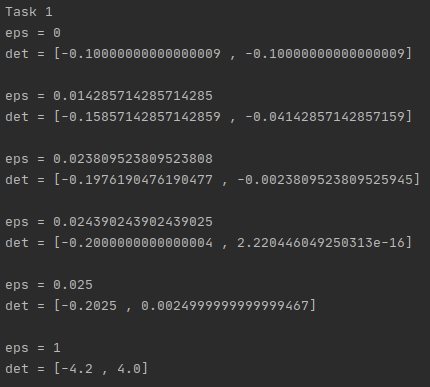
\includegraphics[width=0.75\textwidth]{task_1.png}
	\caption{Определители матриц с заданными $\varepsilon$}
\end{figure}

Результаты численного эксперимента соответствуют полученным аналитически результатам: для значений $[0, \frac{1}{70}, \frac{1}{42}]$ определитель не содержит 0; для значений $[\frac{1}{41}, \frac{1}{40}, 1]$ определитель содержит 0.


\subsection{Задача 2}

\subsubsection{Численный эксперимент}

Очевидно, что при $\varepsilon \geq 1$ матрица является особенной, так как содержит особенную точечную матрицу со всеми элементами - единицами. \\
Попробуем улучшить эту оценку, используя признаки Бекка и Румпа. \\

\textbf{Теорема (признак Бекка)} \\
Пусть интервальная матрица $A \in IR^{n \times n}$ такова, что ее середина $mid A$ неособенна и
\begin{equation}
	\rho(|(mid A)^{-1}| * rad A) < 1
\end{equation}
Тогда A неособенна. \\

\textbf{Теорема (признак Румпа)} \\
Если для интервальной матрицы $A \in IR^{n \times n}$ имеет место
\begin{equation}
	\sigma_{max}(rad A) < \sigma_{min}(mid A)
\end{equation}
Тогда A неособенна. \\

Возьмем начальное значение $\varepsilon = 0.001$ и будем его увеличивать с шагом $0.001$, пока хотя бы один из признаков подтверждает, что матрица является неособенной. Запишем $\varepsilon$ для такой последней матрицы.\\
Размерности матриц возьмем от 2 до 20. \\
Получим следующие результаты:

\begin{figure}[h]
	\centering
	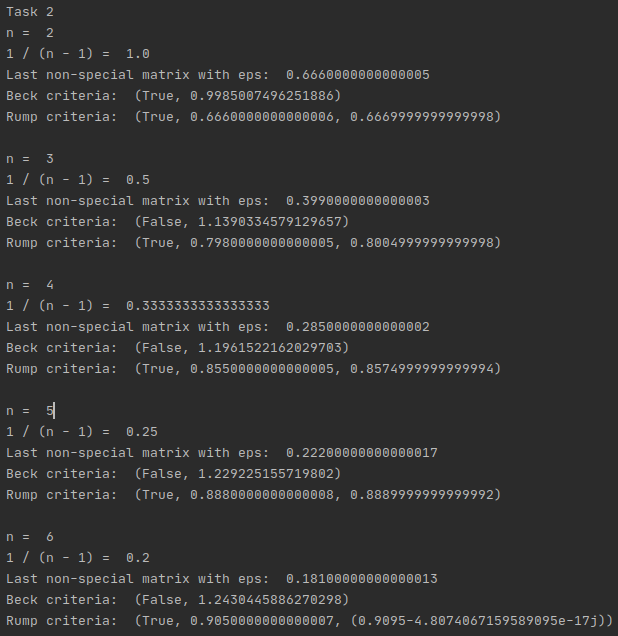
\includegraphics[width=0.75\textwidth]{task_2_1.png}
	\caption{Полученные значения $\varepsilon$ и величины $\frac{1}{n - 1}$}
\end{figure}

\newpage

\begin{figure}[h]
	\centering
	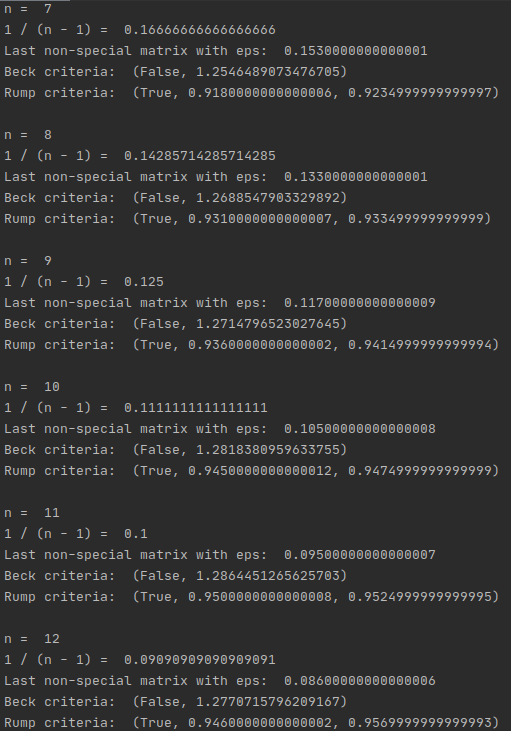
\includegraphics[width=0.75\textwidth]{task_2_2.png}
	\caption{Полученные значения $\varepsilon$ и величины $\frac{1}{n - 1}$}
\end{figure}

\newpage

\begin{figure}[h]
	\centering
	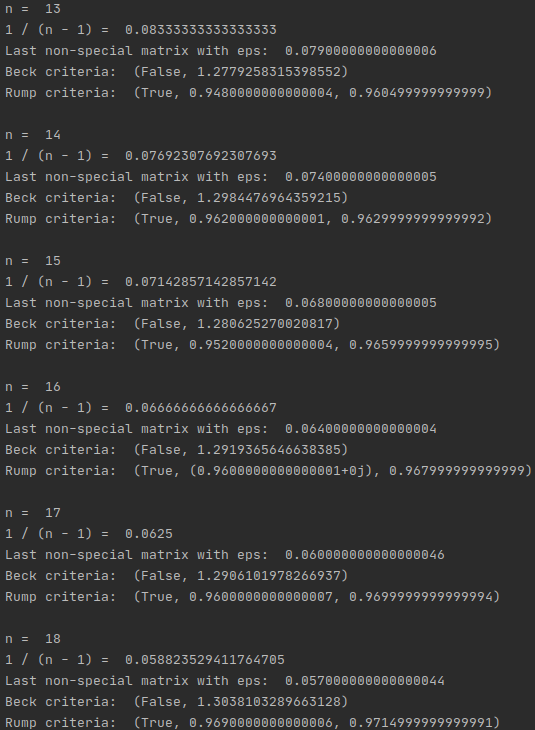
\includegraphics[width=0.75\textwidth]{task_2_3.png}
	\caption{Полученные значения $\varepsilon$ и величины $\frac{1}{n - 1}$}
\end{figure}

\newpage

\begin{figure}[h]
	\centering
	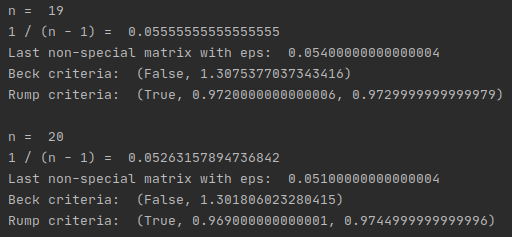
\includegraphics[width=0.75\textwidth]{task_2_4.png}
	\caption{Полученные значения $\varepsilon$ и величины $\frac{1}{n - 1}$}
\end{figure}

Из результатов видно, что полученные $\varepsilon$ немного меньше величин $\frac{1}{n - 1}$, которые можно получить, применив признак Адамара. \\

\textbf{Теорема (интервальный признак Адамара)} \\
Интервальная матрица с диагональным преобладанием является неособенной. \\

Таким образом, можно использовать значения $\varepsilon > \frac{1}{n - 1}$ для получения особенных матриц.


\section{Приложение}
Код программы на Python лежит в данном репозитории: \\
\url{https://github.com/PinkOink/Interval_Analysis/tree/main/lab1}{}


\end{document}